Wintertodt is a skilling boss that is primarily fought (in a manner similar to a minigame moreso than combat) for \texttt{firemaking} experience and resources, either solo or as part of a (large) group. Experience is gained from actions during the fight, with a bonus awarded for players that have contributed enough. The bonus provides experience and \texttt{supply crates} which contain valuable resources.

\begin{figure}
	\centering
	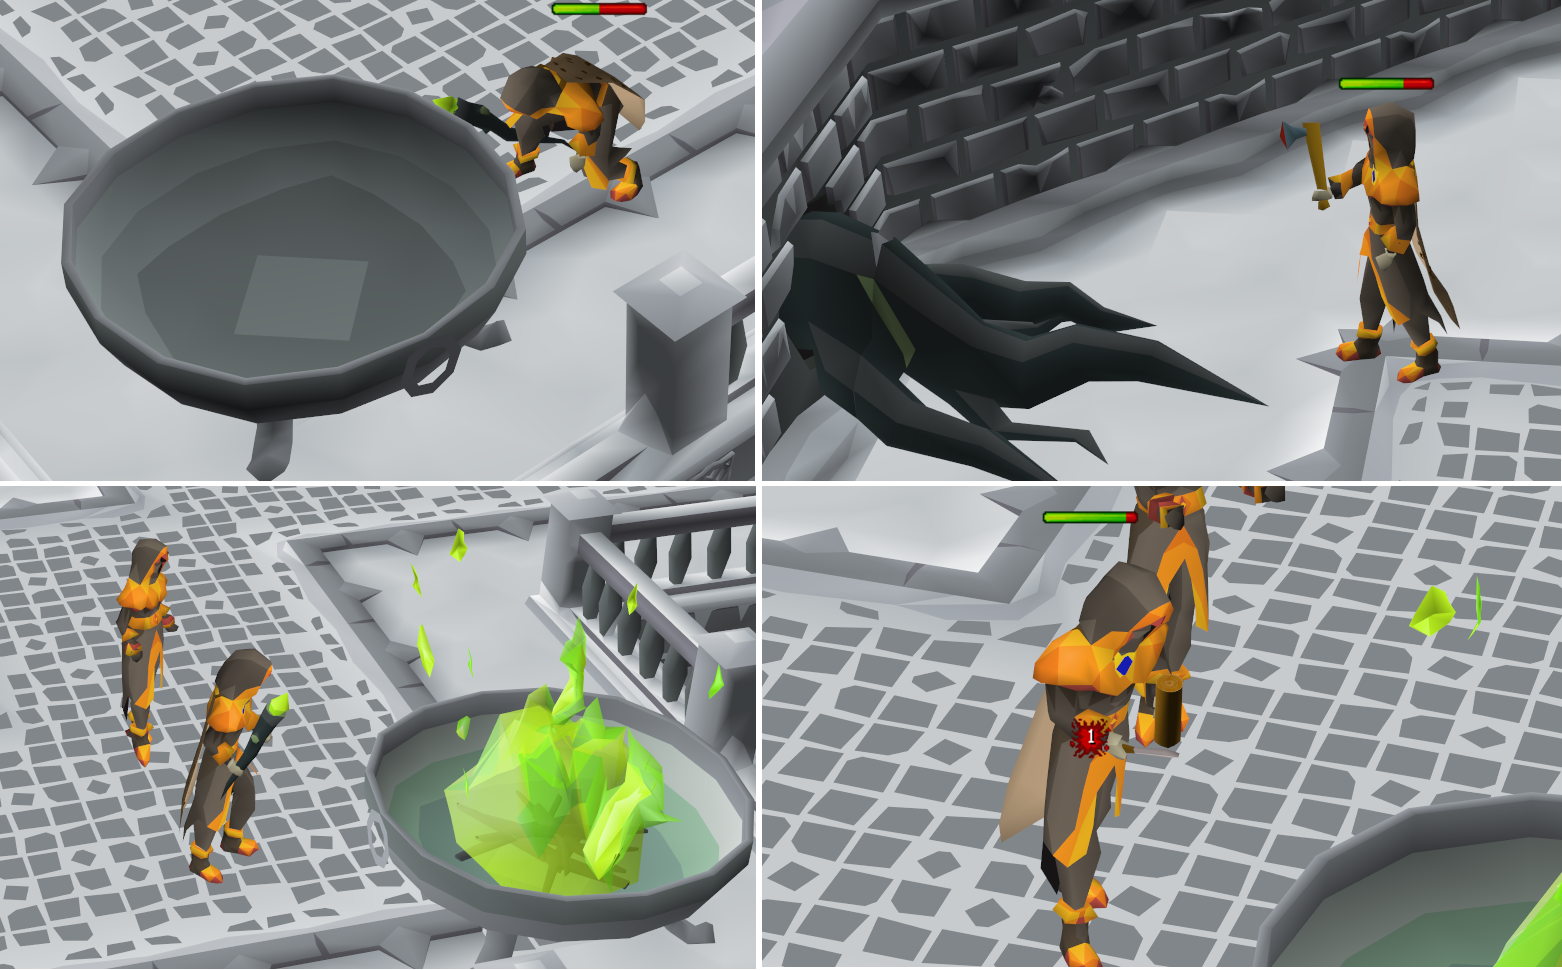
\includegraphics[width=\linewidth]{img/firemaking/wintertodt_actions.png}
	\caption{
		A player performing several actions during a Wintertodt fight. From top-left to bottom-right the player is: lighting a brazier, chopping tree roots, burning roots/kindling, and fletching roots into kindling. Actions that are not shown including creating potions, healing the Pyromancer, and fixing/repairing the brazier.
	}
	\label{fig:wintertodt_actions}
\end{figure}

The objective of the fight is to defeat the \texttt{Wintertodt}. This is done by keeping any of the four braziers lit, which do damage over time to the boss. The players will chop tree roots that can be used to feed the braziers. It should be noted that braziers can be extinguished by the cold wind, regardless of whether the player is feeding it. The roots can optionally be fletched into kindling which provides more experience and points (but requires more time to process). Occasionally, the braziers will break (due to the high temperatures) and the player will have to repair it before relighting it. Finally, each brazier has an associated Pyromancer who may require healing during the fight. In a group setting, many of the required actions can be performed by others (eg: repairing, healing). Several of these actions are shown in Fig.~\ref{fig:wintertodt_actions}.

Most actions award the player with points and provide experience in some skill. The experience scales linearly with the respective skill level, with the proportionality constant determined by action. If the player reaches a threshold of 500 points, they gain bonus experience and a supply crate at the end of a fight. A summary of these actions can be found below in Table.~\ref{table:wintertodt_actions}.
\begin{table}[H]
	\caption{Actions and the associated skills, XP multipliers, and points awarded.}
	\centering
	\begin{tabular}{lcccc}
		\multicolumn{1}{c}{\textbf{Action}} & \textbf{Skill}                                                                   & \textbf{XP Multiplier} (M) & \textbf{Points} \\
		Lighting braziers                   & 
\includegraphics[width=0.03\linewidth]{img/general/skills/Firemaking_icon.png}   & 6.0x                     & 25              \\
		Chopping Root                       & 
\includegraphics[width=0.03\linewidth]{img/general/skills/Woodcutting_icon.png}  & 0.3x                   & -               \\
		Burning Root                        & 
\includegraphics[width=0.03\linewidth]{img/general/skills/Firemaking_icon.png}   & 3.0x                     & 10              \\
		Burning Kindling                    & 
\includegraphics[width=0.03\linewidth]{img/general/skills/Firemaking_icon.png}   & 3.8x                   & 25              \\
		Repairing Brazier                   & 
\includegraphics[width=0.03\linewidth]{img/general/skills/Construction_icon.png} & 4.0x                     & 25              \\
		Healing Pyromancer                  & 
\includegraphics[width=0.03\linewidth]{img/general/skills/blank.png}             & 0.1x                   & 30              \\
		Creating Potion                     & 
\includegraphics[width=0.03\linewidth]{img/general/skills/Herblore_icon.png}     & -                      & -               \\
		Picking Bruma Herb                  & 
\includegraphics[width=0.03\linewidth]{img/general/skills/Farming_icon.png}      & -                      & -               \\
		Win with 500+ Points                & 
\includegraphics[width=0.03\linewidth]{img/general/skills/Firemaking_icon.png}   & 100x                   & -              
	\end{tabular}
	\label{table:wintertodt_actions}
\end{table}

There are several problems that would be interesting to solve. The mechanics and important problems vary depending of whether the boss in fought in a large group (the modeling of which would be quite involved) or solo. For solo fights, the optimal strategy (i.e. which actions to perform when) could be investigated. For large groups, we can ignore the behavior of the group by making certain assumptions. For example, chopping time can be ignored if we assume that the player always reaches a target number of points. We will tackle the latter since group fights are (empirically) more common. The quantities of interest are the number of kills required to obtain a certain level, the number of crates/value/resources obtained after a certain number of kills, and the time required for a kill. For experience, we will only be concerned with firemaking for now.

\section{Large groups}
	We will be attempting to determine the number of games required to get to a desired firemaking level. Since the game play is relatively involved, we will apply a constraint to the player's actions to make it more manageable. We will limit the actions to burning, fletching, and cutting, meaning that healing, relighting, and repairing are ignored. Although this isn't exactly how players would play, only relighting provides firemaking experience, and all ignored actions can be performed by others. Furthermore, all those actions are infrequent in comparison to burning and so these shouldn't be too significant.

	We define $L_\text{FM}$ to be the player's firemaking level. Let $M_\text{root}=3$, $M_\text{kindling}=3.8$, and $M_\text{bonus}=100$ be the XP multiplier for burning a root, burning a kindling, and obtaining 500+ points, respectively. Finally, $P_\text{root}=10$ points are given for burning a root, $P_\text{kindling}=25$ are given for burning kindling. Since the player may level up during a fight (and thereby change their experience rate), we consider this problem in two stages: within fight and outside a fight. Finally, we will need to make use of the level equation, $\mathcal{L}$ from Chapter~\ref{chp:experience_and_levels} that tells us what level a skill is, given its experience.

	\subsection{Within a Fight}
		Since a player may level up during the course of a fight, we need to consider the experience gained on a per action basis. We will label the total player's firemaking experience after $a$ actions are performed as $E_a$. The firemaking actions during a fight come from burning either roots or kindling. To be general, let's define an indicator function $\delta^n_\text{action}$ that is 1 if the $n$'th action performed by the player matches the subscripted value, and is zero otherwise. Then the value of the XP multiplier for the $n$'th firemaking action can be given by:
		\begin{align}
			c_n \equiv \delta_\text{root}^n M_\text{root} + \delta_\text{kindling}^n M_\text{kindling}.
		\end{align}
		Starting with $E_0$ experience, the experience after $a$ actions during a kill is governed by:
		\begin{align}
			E_{n+1} &= E_{n} + c_n\mathcal{L}(E_{n})
		\end{align}
		This equation \emph{may} have a solution except that $\mathcal{L}$ has no analytic form, and so this must be evaluated iteratively. Practically, we can introduce player policies by labeling the coefficients as $c_n^\text{policy}$, where the policy can be, for example, \emph{Only Burning Roots} (OBR) which would be defined as:
		\begin{align}
			c_n^\text{OBR} = M_\text{root}\,\forall n.
		\end{align}
		The labeling $E_{n}^\text{policy}$ may be used to denote the experience gained according to some policy.
		More advanced policies can also be defined. A reasonable strategy to maximize experience while reaching the point threshold would be to burn kindling until the player obtains 500 points followed by burning logs until they reach some target number of points, $T$. We can call this the \emph{Kindle Till Bonus} (KTB) policy, which could be defined as:
		\begin{align}
			c_n^\text{KTB} = \begin{cases}
				M_\text{kindling} &\text{if } n \le 500/P_\text{kindling}\\
				M_\text{root} &\text{if } n \le \frac{T}{P_\text{root}} - \frac{P_\text{kindling}}{P_\text{root}}\lceil 500/P_\text{kindling} \rceil \\
				0 & \text{otherwise}.
			\end{cases}
		\end{align}
		The first bound is the number of kindling needed to reach 500 points. The second bound is the number of points remaining, divided by the points per root which gives the number of roots left.


	\subsection{Across Fights}
		We now have the ability to calculate the firemaking experience gained during a fight (under some constraints). We can take this further to calculate the firemaking experience gained across fights. The experience that a player has after $k$ kills can be denoted as $\mathcal{E}^k$. There are two contributions for this, one is the experience that a player gains during a fight, the other is the bonus experience gained after a kill. And so,
		\begin{align}
			\mathcal{E}^{k+1} &= \mathcal{E}^k + \mathcal{E}_{N(T; \text{policy})}^\text{policy} + \theta(T - 500)M_\text{bonus}L_\text{fm},
		\end{align}
		where $N(T; \text{policy})$ is the number of actions to perform given the target and policy, and $\theta$ is the Heaviside step function. This equation can again only be evaluated numerically. 
